\chapter{Design}

\section{Architettura}
L’architettura di MPoly è basata sul pattern architetturale MVC.
Si è scelto di implementare l’architettura nella sua forma classica in quanto il gioco 
ha una modalità di interazione prettamente statica: l’utente interagisce con la view, 
facendo scaturire un evento; a seguito di questo evento si eseguono una serie di operazioni 
specifiche per la sua gestione con conseguente aggiornamento della view, che mostra all’utente che cosa è successo.   
È stato predisposto un controller principale denominato GameManager. 
Questo implementa il pattern observer e si mette in ascolto degli eventi che vengono catturati dalla view. 
Nel momento in cui viene notificato di un evento il controller interroga il model.
La componente model dell'applicazione ha dei determinati punti d'entrata. 
Nello specifico abbiamo Board, che si occupa di gestire la struttura e lo stato del tabellone,
TurnationManager, che si occupa di gestire l’avanzamento della partita, l'avvicendarsi dei turni dei giocatori e il tiro dei dadi, 
e Bank, per gestire lo scambio di denaro e la compravendita delle proprietà. 
Questi punti d’ entrata del model offrono delle primitive che incapsulano la logica di funzionamento 
delle principali azioni che si possono compiere durante il gioco. Queste azioni sono caratteristiche del 
gioco stesso Monopoly. 
Con questa architettura il model è perfettamente scorporabile e utilizzabile per costruire 
un software diverso che risponda allo stesso dominio. 
Una volta finita l’interrogazione del model il GameManager si occuperà di chiamare 
delle funzioni sulla view che aggiornano il contenuto di quest’ultima. 
Il controller agisce su model e view mediante delle interfacce che sono completamente indipendenti 
dall’implementazione di quest’ultimi. 
Questo, in particolare, fa sì che la modalità di implementazione della view non determini cambiamenti sul 
controller o sul model in alcun caso. 
Il software prevede anche un menù iniziale di configurazione della partita. 
Questo menù è a sua volta costituito da una sua architettura MVC più ridotta, 
modellata tenendo in mente gli stessi principi descritti sovrastante. 
L’entità GameBuilder è colei che si occupa di instanziare poi le classi dell’MVC principale del software e avviare effettivamente il gioco,
costruendo tutti gli oggetti.

\begin{figure}[H]
    \centering
    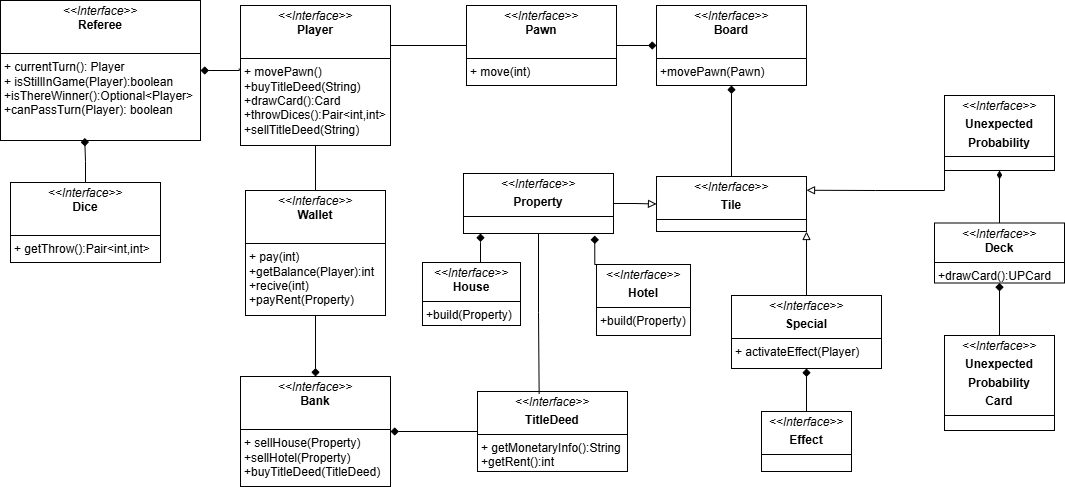
\includegraphics[width=0.5\textheight]{img/architecture_diagram1.png}
    \caption{SCHEMA SBAGLIATO}
	\label{img:architecture_diagram1}
\end{figure}
